% =====================================================================
%  GenomIO: A Three Node Multi-Agent System for Genomic Gap Filling
%  Thesis chapter. Compile with:  pdflatex multiagent_system.tex  (twice)
% =====================================================================
\documentclass[11pt,a4paper]{article}

\usepackage[utf8]{inputenc}
\usepackage[T1]{fontenc}
\usepackage[english]{babel}
\usepackage[margin=2.5cm]{geometry}
\usepackage{graphicx}
\usepackage{booktabs}
\usepackage{multirow}
\usepackage{xcolor}
\usepackage{listings}
\usepackage{amsmath}
\usepackage{amssymb}
\usepackage{tikz}
\usepackage{caption}
\usepackage{float}
\usepackage[hidelinks]{hyperref}

\usetikzlibrary{arrows.meta,positioning,calc,fit,backgrounds,shapes.geometric}

% =============================================================== colours
\definecolor{codebg}{RGB}{248,248,246}
\definecolor{codeframe}{RGB}{210,210,205}
\definecolor{kw}{RGB}{0,90,160}
\definecolor{str}{RGB}{160,60,30}
\definecolor{cmt}{RGB}{110,120,110}
\definecolor{nodeA}{RGB}{222,235,247}
\definecolor{nodeB}{RGB}{226,240,226}
\definecolor{nodeC}{RGB}{250,238,222}
\definecolor{edgecol}{RGB}{60,60,60}

% =============================================================== listings
\lstdefinestyle{py}{
  language=Python,
  backgroundcolor=\color{codebg},
  basicstyle=\ttfamily\footnotesize,
  keywordstyle=\color{kw}\bfseries,
  stringstyle=\color{str},
  commentstyle=\color{cmt}\itshape,
  numbers=left, numberstyle=\tiny\color{gray}, numbersep=8pt,
  frame=single, rulecolor=\color{codeframe},
  breaklines=true, breakatwhitespace=true,
  showstringspaces=false,
  captionpos=b,
  xleftmargin=14pt, framexleftmargin=14pt,
  tabsize=4,
}
\lstdefinestyle{sh}{
  language=bash,
  backgroundcolor=\color{codebg},
  basicstyle=\ttfamily\footnotesize,
  keywordstyle=\color{kw},
  commentstyle=\color{cmt}\itshape,
  frame=single, rulecolor=\color{codeframe},
  breaklines=true, showstringspaces=false, captionpos=b,
  xleftmargin=6pt, framexleftmargin=6pt,
}
\lstdefinestyle{js}{
  backgroundcolor=\color{codebg},
  basicstyle=\ttfamily\footnotesize,
  stringstyle=\color{str},
  frame=single, rulecolor=\color{codeframe},
  breaklines=true, showstringspaces=false, captionpos=b,
  xleftmargin=6pt, framexleftmargin=6pt,
}
\lstset{style=py}

\newcommand{\code}[1]{\texttt{\small #1}}

% =====================================================================
\title{\textbf{A Three Node Multi-Agent System for\\Genomic Gap Filling}\\[4pt]
       \large Design, Implementation and Evaluation on the ARES Cluster}
\author{GenomIO}
\date{August 2026}

\begin{document}
\maketitle

\begin{abstract}
\noindent
This chapter describes the redesign of the GenomIO gap filling pipeline as a multi-agent
system. The previous version was a single process that chained retrieval and
prediction together through a language model. The new version is three independent agents, each running on
its own compute node of the ARES cluster, communicating over the Agent2Agent (A2A)
protocol, with every capability exposed as a Model Context Protocol (MCP) tool.

Each agent hosts a \emph{surrogate model}, a trained network standing in for a
computation that is exact but too slow to perform directly. The retrieval agent holds two:
DNABERT-S, which replaces letter by letter sequence alignment with a comparison of short
numeric vectors, and an approximate nearest neighbour index which replaces exhaustive
search over 43{,}575 references. The reconstruction agent holds GENA-LM, which stands in
for the unknown true sequence. The language model inside each agent performs none of this
work; it decides when the surrogates are invoked and with what parameters.

The motivation was not distribution for its own sake. The previous pipeline contained a
defect that no test could detect: the reference sequences it retrieved were silently
discarded before the prediction model ever saw them, while the run was still recorded as
retrieval augmented. The cause was that the component knowing the model's input budget and
the component choosing the references were the same function, so the constraint linking
them was never written down. Separating them onto different machines forces that quantity
into a message, where it is necessarily measured and recorded.

Running the same test case as the original pipeline, gap number one of accession
AP012051.1, the new system reports that 2{,}942 tokens of retrieved reference sequence
reached the prediction model, out of a measured budget of 3{,}236. The previous pipeline
reported nothing, and would have delivered zero.

The improvements are infrastructural and are set out in Section~\ref{sec:mas}. They fall
into two groups: those that follow from having specific agents, such as a budget that must
cross an interface and therefore gets recorded, rules enforced at that interface, failures
that stay where they happen and a run that can be audited across machines; and those that
follow from each agent owning the specific models its role requires, such as searches that
run 83 times faster because the embedder is already resident, and three components with
very different memory and startup costs each receiving a node that suits it.
\end{abstract}

\tableofcontents
\newpage

% =====================================================================
\section{The problem, in plain terms}
\label{sec:problem}

\subsection{What a genome gap is}

A genome is a very long text written in an alphabet of four letters: A, C, G and T. When
biologists sequence an organism, the machine cannot read the whole text at once. It reads
many short fragments, and software then assembles those fragments into longer pieces
called \emph{contigs}, from the word contiguous.

The assembly is rarely complete. Between two neighbouring contigs there is often a
stretch that no fragment covered. That stretch is a \emph{gap}. We know roughly how long
it is, we know the sequence immediately to its left and to its right, but we do not know
what letters go inside it.

\begin{center}
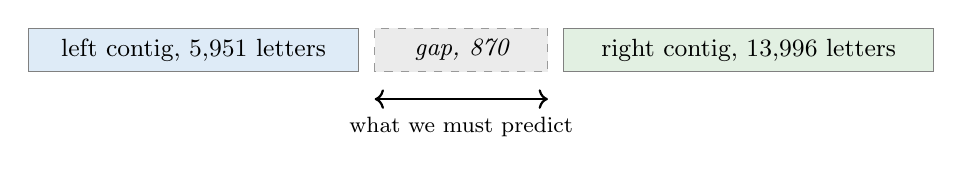
\begin{tikzpicture}[scale=1]
  \draw[fill=nodeA,draw=black!50] (0,0) rectangle (4.2,0.55);
  \node at (2.1,0.275) {\small left contig, 5{,}951 letters};
  \draw[fill=black!8,draw=black!40,dashed] (4.4,0) rectangle (6.6,0.55);
  \node at (5.5,0.275) {\small\itshape gap, 870};
  \draw[fill=nodeB,draw=black!50] (6.8,0) rectangle (11.5,0.55);
  \node at (9.15,0.275) {\small right contig, 13{,}996 letters};
  \draw[<->,thick] (4.4,-0.35) -- (6.6,-0.35);
  \node at (5.5,-0.7) {\footnotesize what we must predict};
\end{tikzpicture}
\end{center}

\emph{Gap filling} is the task of predicting the missing letters. Throughout this chapter
the running example is the first gap of the bacterial genome with accession AP012051.1.
It is 870 letters long, it sits between two contigs of 5{,}951 and 13{,}996 letters, and
because this is a simulated draft genome we know the true answer and can check any
prediction against it.

\subsection{How a language model can help}

Two ideas are combined.

The first is a \textbf{prediction model}. GENA-LM is a neural network trained on DNA in
the same way that a text model is trained on English: hide some letters and learn to
guess them from the surrounding context. To fill a gap we hand it the left contig, a run
of blanks, and the right contig, and ask it to fill the blanks. Its input is limited to
4{,}096 \emph{tokens}, where a token is a short group of letters that the model treats as
one unit. In our data one token is worth roughly six letters of DNA.

The second is \textbf{retrieval}. Before predicting, we look in a reference library of
43{,}575 known genes for sequences that resemble the region around the gap, and we place
those in the model's input as extra evidence. The reasoning is that a gene similar to the
one being reconstructed tells the model what such a sequence usually looks like. Finding
similar sequences quickly is done by converting each one into a list of 768 numbers, an
\emph{embedding}, using a model called DNABERT-S, and then searching for the closest
lists with a library called FAISS. This combination of retrieval and generation is
commonly called RAG, for retrieval augmented generation.

The whole difficulty of this chapter lies in one sentence: \textbf{the retrieved evidence
is only useful if it actually reaches the prediction model}, and in the previous system
it did not.

% =====================================================================
\section{The previous pipeline}
\label{sec:old}

\subsection{What it was}

The earlier system was a single Python process built with the LangChain library. A user
called a function \code{plan()} with the sequence and the gap length. That function
created an \emph{agent}: a language model, Gemini 2.5 Flash, given a written instruction
and two tools it could choose to call.

\begin{figure}[H]
\centering
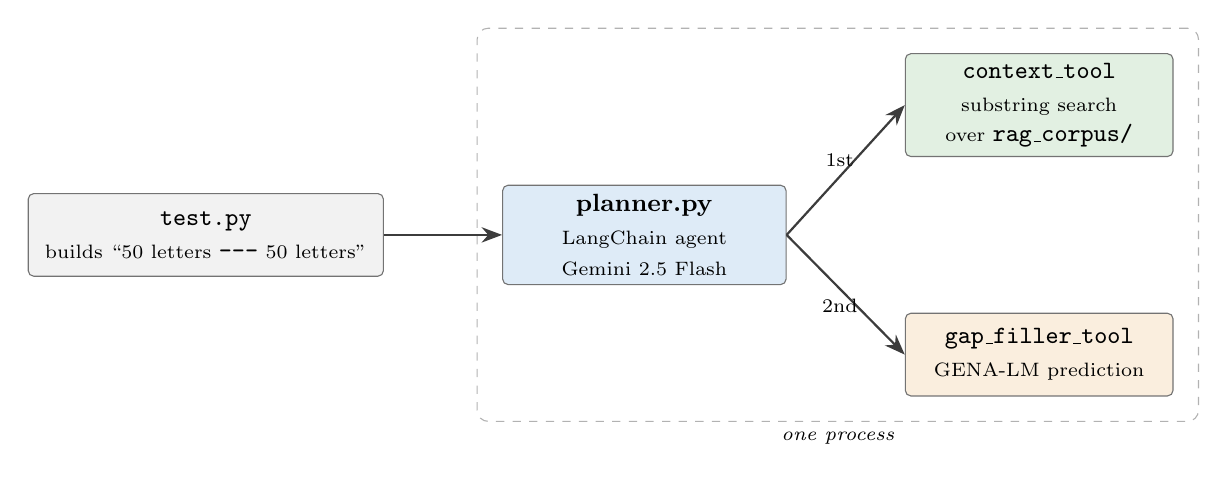
\begin{tikzpicture}[
  box/.style={draw=black!55, rounded corners=2pt, align=center,
              minimum height=1.05cm, inner xsep=6pt, font=\small},
  ar/.style={-{Stealth[length=2.6mm]}, thick, draw=edgecol},
]
  \node[box, fill=black!5, minimum width=3.1cm] (t) {\code{test.py}\\[1pt]
        \scriptsize builds ``50 letters \code{-{}-{}-} 50 letters''};
  \node[box, fill=nodeA, minimum width=3.6cm, right=1.5cm of t] (p)
        {\textbf{planner.py}\\[1pt]\scriptsize LangChain agent\\\scriptsize Gemini 2.5 Flash};
  \node[box, fill=nodeB, minimum width=3.4cm, above right=0.35cm and 1.5cm of p] (r)
        {\code{context\_tool}\\[1pt]\scriptsize substring search\\\scriptsize over \code{rag\_corpus/}};
  \node[box, fill=nodeC, minimum width=3.4cm, below right=0.35cm and 1.5cm of p] (g)
        {\code{gap\_filler\_tool}\\[1pt]\scriptsize GENA-LM prediction};

  \draw[ar] (t) -- (p);
  \draw[ar] (p.east) -- node[above,font=\scriptsize,pos=0.45]{1st} (r.west);
  \draw[ar] (p.east) -- node[below,font=\scriptsize,pos=0.45]{2nd} (g.west);

  \begin{scope}[on background layer]
    \node[draw=black!30, dashed, rounded corners, fit=(p)(r)(g),
          inner sep=9pt, label={[font=\scriptsize\itshape]below:one process}] {};
  \end{scope}
\end{tikzpicture}
\caption{The previous pipeline. One process, one language model, two tools. The ordering
of the two tool calls was requested in the written instruction, not enforced.}
\label{fig:old}
\end{figure}

The written instruction said, in part:

\begin{quote}\ttfamily\small
You MUST use these tools in the correct order:\\
1) context\_tool\\
2) gap\_filler\_tool
\end{quote}

\subsection{Why it did not work}

Five problems were found by inspection and by measurement. They are listed here because
each one motivates a specific decision in the new design.

\paragraph{1. The ordering was a request, not a rule.}
The instruction above is ordinary English addressed to a language model. Nothing in the
code checked it. The LangChain executor imposed no ordering, set no limit on the number
of steps and had no failure handling. The model could have called the prediction tool
without retrieving anything, or looped, and nothing would have noticed.

\paragraph{2. The DNA travelled through the language model.}
The nucleotide string was written into the prompt, and the model was expected to type it
back out as an argument to the second tool. The scientific payload therefore passed
through text generation, with no checksum and no length check. At the 50 letter flanks
actually used this survived, but nothing guaranteed it.

\paragraph{3. Retrieval found nothing.}
The retrieval tool did not perform a similarity search. It used Python's \code{in}
operator, so a reference gene counted as a match only if the query appeared inside it
character for character. Measured against the real query for gap number one, over the
whole 37{,}645 record library:

\begin{center}
\begin{tabular}{lcc}
\toprule
Query flank length & Records containing both flanks & Records containing either \\
\midrule
50 letters & 0 & 0 \\
20 letters & 0 & 0 \\
12 letters & 1 & 18 \\
\bottomrule
\end{tabular}
\end{center}

At the 50 letter flank the pipeline actually used, retrieval returned nothing at all. The
retrieval augmented arm of the experiment was therefore identical to the arm without
retrieval, though the results were labelled otherwise.

\paragraph{4. The retrieved evidence was discarded before the model saw it.}
This is the most consequential problem, and it lived in the standalone comparison script
rather than the agent. The input was assembled as
\begin{center}
\code{\{left contig\} [MASKS] \{right contig\}}\verb|\n\n|\code{\# Context: \{retrieved\}}
\end{center}
and then tokenised with truncation enabled at 4{,}096 tokens. Truncation removes from the
\emph{end}. The retrieved evidence was therefore the first thing deleted. No error was
raised; the run completed and the result was recorded as retrieval augmented.

\paragraph{5. The test selected the wrong contigs.}
The test script took the first and second entries of the contig file. That file is sorted
from longest to shortest, so the first two entries are contig number 31 (190{,}651
letters, at genome position 1{,}298{,}041 to 1{,}488{,}692) and contig number 22
(167{,}069 letters, at position 898{,}138 to 1{,}065{,}207). These two are not adjacent
to each other and have no gap between them. They were nonetheless passed alongside the
870 letter target belonging to gap number one, whose true neighbours are contig number 1
and contig number 2.

\subsection{The state of the code}

Independently of the design, the previous pipeline could not be executed at all. The
retrieval module opened a directory named \code{rag/rag\_corpus}, which does not exist
(the library is at \code{rag\_corpus} in the project root), so the first tool call raised
a file not found error. The test script read the data from a path missing its
\code{data/} prefix. The three modules required three mutually incompatible import roots.
The LangChain packages were not installed and no API key was configured.

% =====================================================================
\section{The new system}
\label{sec:new}

\subsection{The central idea}

The fourth problem above, the discarded evidence, has a specific cause. The component
that knows the token budget (the prediction model) and the component that chooses the
reference sequences (the retrieval search) were the same piece of code. Because there was
no boundary between them, the constraint linking them was never written down. The number
of sequences retrieved was a constant, \code{k = 2}, chosen with no reference to how much
room the model actually had.

The new design separates them into different processes on different machines. Once they
are apart, they cannot share the assumption implicitly. They have to exchange it, and the
exchange is measurable.

\begin{quote}
\textbf{Neither agent can answer the question alone.} Retrieval knows which reference
sequences are most similar, but not how much space is left in the prediction model's
input. Reconstruction knows exactly how much space is left, but has no access to the
reference library. The answer to ``how many references fit?'' must be negotiated.
\end{quote}

\subsection{The three agents}

\begin{description}
\item[Coordinator.] Executes policy, not science. It loads no models. It cuts the query
  out of the two contigs, checks that its two peers are alive and reading the same
  reference library, delegates the work, and applies an acceptance check to whatever
  comes back.
\item[Retrieval agent.] Owns DNABERT-S and the FAISS index of 43{,}575 reference genes.
  It answers a request for candidates with \emph{row numbers and similarity scores},
  never with DNA.
\item[Reconstruction agent.] Owns GENA-LM. Because it owns the model, it is the only
  component that can measure the token budget, so it drives the negotiation and performs
  the final prediction.
\end{description}

\begin{figure}[H]
\centering
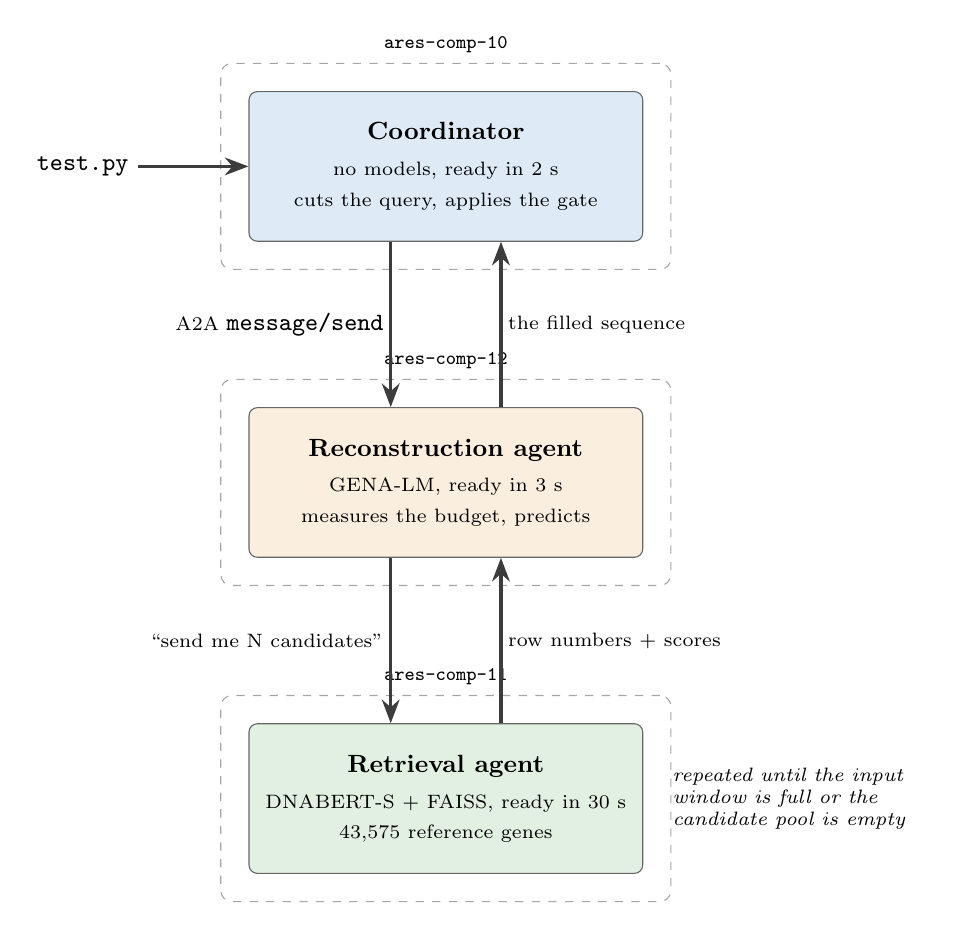
\begin{tikzpicture}[
  node distance=1cm,
  agent/.style={draw=black!60, rounded corners=3pt, align=center,
                minimum width=5.0cm, minimum height=1.9cm, font=\small},
  machine/.style={draw=black!35, dashed, rounded corners=4pt, inner sep=10pt},
  ar/.style={-{Stealth[length=3mm]}, very thick, draw=edgecol},
  lbl/.style={font=\scriptsize, fill=white, inner sep=2pt},
]
  \node[agent, fill=nodeA] (co)
    {\textbf{Coordinator}\\[2pt]
     \scriptsize no models, ready in 2 s\\
     \scriptsize cuts the query, applies the gate};
  \node[agent, fill=nodeC, below=2.1cm of co] (re)
    {\textbf{Reconstruction agent}\\[2pt]
     \scriptsize GENA-LM, ready in 3 s\\
     \scriptsize measures the budget, predicts};
  \node[agent, fill=nodeB, below=2.1cm of re] (rt)
    {\textbf{Retrieval agent}\\[2pt]
     \scriptsize DNABERT-S + FAISS, ready in 30 s\\
     \scriptsize 43{,}575 reference genes};

  \node[machine, fit=(co), label={[font=\scriptsize\ttfamily]above:ares-comp-10}] {};
  \node[machine, fit=(re), label={[font=\scriptsize\ttfamily]above:ares-comp-12}] {};
  \node[machine, fit=(rt), label={[font=\scriptsize\ttfamily]above:ares-comp-11}] {};

  \draw[ar] ($(co.south)+(-0.7,0)$) -- node[lbl,left]{A2A \code{message/send}}
            ($(re.north)+(-0.7,0)$);
  \draw[ar] ($(re.north)+(0.7,0)$) -- node[lbl,right]{the filled sequence}
            ($(co.south)+(0.7,0)$);

  \draw[ar] ($(re.south)+(-0.7,0)$) -- node[lbl,left]{``send me N candidates''}
            ($(rt.north)+(-0.7,0)$);
  \draw[ar] ($(rt.north)+(0.7,0)$) -- node[lbl,right]{row numbers + scores}
            ($(re.south)+(0.7,0)$);

  \node[font=\scriptsize\itshape, right=0.25cm of rt.east, text width=3.1cm]
       {repeated until the input window is full or the candidate pool is empty};

  \node[left=1.4cm of co, font=\small] (user) {\code{test.py}};
  \draw[ar] (user) -- (co);
\end{tikzpicture}
\caption{The three node deployment. Each agent runs on its own ARES compute node. The
double arrow between reconstruction and retrieval is the negotiation, and it repeats
several times per run.}
\label{fig:new}
\end{figure}

\subsection{How the agents talk: A2A}

The Agent2Agent protocol defines how one agent asks another to do something. It is
ordinary HTTP with JSON messages, which is why no message broker or central server is
needed. Three parts of it matter here.

\paragraph{The agent card.} Every agent publishes a description of itself at a fixed
address, \code{/.well-known/agent-card.json}. It states the agent's name, what it can do
(its \emph{skills}), and which optional protocol features it supports. Our agents also
publish a fingerprint of the reference library they are reading, which the coordinator
compares between the two peers before delegating. If they disagree, a row number would
mean a different gene to each of them, and every result would be wrong in a way nothing
would detect.

\paragraph{Tasks.} A unit of work is a \emph{task} with an identity and a lifecycle. The
protocol defines nine states; our agents move through \code{submitted}, \code{working}
and then either \code{completed} or \code{failed}. A finished task can never be restarted,
which is what makes a run auditable afterwards.

\paragraph{Messages and artifacts.} A request carries \emph{parts}. We use two kinds: a
\code{DataPart} holding structured JSON, and a \code{TextPart} holding prose. The result
comes back as an \emph{artifact} containing both. Everything the system actually depends
on travels in the \code{DataPart}. The prose is advisory, and the reason for that
separation is explained in Section~\ref{sec:invariants}.

\begin{lstlisting}[style=js,caption={A request from the coordinator to the reconstruction
agent, abbreviated. The contigs travel as structured data, never as prose.}]
{"jsonrpc": "2.0", "id": "req-4f1c", "method": "message/send",
 "params": {"message": {
     "role": "user",
     "messageId": "msg-9a2e",
     "contextId": "ctx-1b7d",
     "parts": [{"kind": "data", "data": {
         "op": "reconstruct",
         "gap_id": "AP012051.1_gap1",
         "gap_length": 870,
         "left":  "TATTATCTTTCCGTTTGGCACAATT...",
         "right": "ATTGGCATTAAACCAGACATTGAAG...",
         "organism": ""}}]}}}
\end{lstlisting}

\subsection{What the agents can do: MCP tools}

Inside each agent runs a language model, and everything that model is able to do is
declared as a Model Context Protocol tool. A tool is a name, a description written for
the model, a parameter schema, and a function. The model reads the descriptions and
decides which to call and when.

\begin{lstlisting}[style=py,caption={An MCP tool. The description is the model's only
instruction manual, so it is written for a reader, not as documentation.}]
@tool(
    "measure_budget",
    "Tokenize the model input with the context slot empty and report how many of the "
    "4096 token positions are free for retrieved context. Must be called before "
    "requesting or admitting any candidates.",
    {"task_id": str},
)
@guarded("measure_budget", requires=None)
async def measure_budget(args: dict, state: ReconTask) -> dict:
    base = mlm.build_model_input("", state.model_left, state.model_right)
    base_tokens = await run_blocking(mlm.count_tokens, tokenizer, base)
    free = config.MAX_LENGTH - base_tokens - seed - config.SAFETY_TOKENS
    state.free_tokens_remaining = max(0, free)
    state.advance(Phase.MEASURED)
    return errors.tool_ok({"base_tokens": base_tokens, "free_tokens": free, ...})
\end{lstlisting}

The complete set is thirteen tools across the three agents:

\begin{center}
\begin{tabular}{lll}
\toprule
Agent & Tool & What it does \\
\midrule
Coordinator & \code{prepare\_query} & cut the query, verify the peers \\
            & \code{delegate\_reconstruction} & hand the task on and wait \\
            & \code{evaluate\_result} & apply the acceptance check \\
            & \code{emit\_trace} & produce the run record \\
\midrule
Retrieval   & \code{retrieve\_context} & open a ranked pool, serve the first batch \\
            & \code{extend\_context} & serve the next batch, no new search \\
            & \code{describe\_rows} & metadata for rows already served \\
\midrule
Reconstruction & \code{measure\_budget} & how many tokens are free \\
            & \code{request\_candidates} & ask retrieval for a batch \\
            & \code{extend\_candidates} & ask for more \\
            & \code{admit\_candidates} & tokenise each, keep what fits \\
            & \code{generate} & run the prediction \\
            & \code{report\_state} & read only diagnostic \\
\bottomrule
\end{tabular}
\end{center}

% =====================================================================
\section{The surrogate models inside the agents}
\label{sec:surrogate}

\subsection{What a surrogate model is}

A \emph{surrogate model} is a learned stand in for a computation that could in principle
be done exactly, but that would be far too slow to do at the scale required. Instead of
performing the exact calculation, a neural network is trained to approximate its answer,
and the approximation is used in its place.

This system contains three surrogates. Two of them live inside the retrieval agent and
one inside the reconstruction agent. None of them is the language model that drives the
agent, and that distinction is the point of this section: \textbf{the language model
schedules the work, the surrogate models perform it}.

\subsection{The two surrogates in the retrieval agent}

\paragraph{DNABERT-S, a surrogate for sequence alignment.}
The exact way to ask whether two DNA sequences are related is to align them, letter by
letter, allowing for insertions and deletions. This is accurate and it is expensive:
comparing one 1{,}800 letter query against 43{,}575 reference genes means tens of millions
of letter comparisons for a single question.

DNABERT-S replaces that. It converts any DNA sequence into a fixed list of 768 numbers,
an embedding, chosen so that related sequences receive similar lists. Asking whether two
sequences are related then becomes a dot product of two short vectors instead of an
alignment of two long strings. The model was trained \emph{contrastively}, which means it
was shown pairs of sequences and taught to pull sequences from the same organism together
and push sequences from different organisms apart. That is precisely the property a
similarity search needs, and it is why this model was selected over fifteen others in the
earlier benchmark.

\paragraph{FAISS HNSW, a surrogate for exhaustive search.}
Even with embeddings, answering ``which of the 43{,}575 references is closest?'' exactly
requires 43{,}575 comparisons. FAISS builds a navigable graph over the embeddings and
walks it greedily, visiting only a small fraction of the records. This is an
\emph{approximate} nearest neighbour search: it usually finds the closest records, and it
is not guaranteed to.

The approximation is visible in the implementation. When the search is restricted to a
single organism, handing the graph a scattered list of permitted records causes the walk
to fail entirely and return nothing at all, because the traversal cannot reach enough
permitted nodes from its entry point. The system therefore searches broadly and filters
afterwards, which is slower but reliable. This is the ordinary cost of using a surrogate:
it must be used within the conditions where its approximation holds.

\subsection{The surrogate in the reconstruction agent}

GENA-LM plays the same role for generation. The exact answer to ``what letters are in this
gap?'' can only be obtained by sequencing the organism again. GENA-LM is a stand in: a
network trained on large quantities of real DNA which, given the surrounding sequence,
produces the letters that would most plausibly appear there. It approximates that
sequence rather than recovering it, which is why the acceptance check in
Section~\ref{sec:gate} tests the delivery of evidence and the shape of the output rather
than biological correctness.

\subsection{Why each surrogate lives inside a specific agent}

Each surrogate is loaded once, when its agent starts, and stays resident in that process
for the lifetime of the deployment. This is not an optimisation detail; it determines
what the architecture can do.

\begin{center}
\begin{tabular}{llrr}
\toprule
Agent & Surrogate held & Load cost & Resident memory \\
\midrule
Retrieval & DNABERT-S embedder & 33.9 s & \multirow{2}{*}{1.0 GB} \\
          & FAISS graph over 43{,}575 genes & 5.5 s & \\
Reconstruction & GENA-LM generator & 2.3 s & 1.2 GB \\
Coordinator & none & 0 s & 0.12 GB \\
\bottomrule
\end{tabular}
\end{center}

The consequence is measurable. A search that must load DNABERT-S first takes 33.9 seconds.
The same search against an already loaded model takes 0.41 seconds, which is \textbf{83
times faster}. In the previous pipeline the generator was reloaded on every invocation of
the processing function, and the substring retriever re read all 51 megabytes of the
reference library from disk on every single call, taking about one second each time. Under
the new arrangement the per request loading cost is zero, because nothing is loaded per
request.

Placement follows from these numbers as well. The retrieval agent needs a full gigabyte and
half a minute of startup; the coordinator needs neither. Giving each its own node means the
coordinator is ready in two seconds and can begin checking on its peers while they are
still loading, and the two memory hungry agents never compete for the same machine's memory
bandwidth.

\subsection{Checking that a surrogate is behaving}

Because a surrogate only approximates, it can be subtly wrong in ways that produce
plausible output. The retrieval surrogate was therefore verified directly, by searching
the index with a reference sequence that is already inside it and checking that the search
returns that same record:

\begin{center}
\begin{tabular}{lll}
\toprule
Query & Its organism & Top three results \\
\midrule
record 23500 & \emph{Fusobacterium animalis} & itself \textbf{1.000}, \emph{F. polymorphum} 0.893, 0.887 \\
record 27000 & \emph{F. polymorphum} & itself \textbf{1.000}, \emph{F. animalis} 0.917, 0.866 \\
record 12500 & \emph{Staphylococcus aureus} & itself \textbf{1.000}, \emph{S. aureus} 0.826, 0.794 \\
\bottomrule
\end{tabular}
\end{center}

A similarity of exactly 1.000 for an identical sequence confirms the whole chain: the
embedder runs, the vectors are normalised the same way they were when the index was built,
the distance is converted back to a similarity correctly, and record number $k$ in the
index really is record number $k$ in the library. Neighbouring records from a related
species scoring 0.89 to 0.92 confirms that the contrastive training is doing its job.

\subsection{The language model is not a surrogate}

It is worth being explicit, because the two are easily confused. Each agent also contains
a general purpose language model, and its role is entirely different. It never embeds a
sequence, never searches the index and never predicts a nucleotide. It reads the
descriptions of the tools available to it and decides which to call and with what batch
size. Every scientific quantity in the final result was computed by a surrogate model or
by ordinary arithmetic, and none of it was produced by the language model. That separation
is enforced by the rules in Section~\ref{sec:invariants}.

% =====================================================================
\section{The three rules that make it trustworthy}
\label{sec:invariants}

Putting a language model in charge of the sequence of operations reintroduces exactly the
weakness described in Section~\ref{sec:old}: a model may skip a step or invent a value.
Three rules prevent that, and none of them is a written instruction.

\subsection{Rule 1: the answer is read from memory, never from the model's words}

Each tool writes its results into a per task record held in the agent's memory. When the
model's turn ends, the reply is assembled by ordinary code from that record. The model's
prose is attached to the artifact and read by nothing.

This is not a theoretical safeguard. During development one retrieval run ended with the
model producing an error message instead of a summary, \emph{after} its tool had already
executed. The task still completed correctly with the right row numbers, because the
answer never depended on what the model said.

\subsection{Rule 2: ordering is a data dependency, not an instruction}

Every tool begins with a check of the task's state, and refuses to do any work if the
prerequisites are missing. The refusal is a structured value that names the exact tool
to call instead.

\begin{lstlisting}[style=js,caption={What the model receives if it tries to admit
reference sequences before measuring the budget. The remedy field is generated at the
moment of the violation by code that knows the true state.}]
{"error": "PRECONDITION_FAILED",
 "code": "BUDGET_NOT_MEASURED",
 "phase": "CREATED",
 "required_phase": "MEASURED",
 "remedy": "Call mcp__reconstruction_agent__measure_budget with this task_id first; "
           "it reports how many tokens are free for retrieved context."}
\end{lstlisting}

The most important of these checks concerns the budget itself. To admit reference
sequences, the model must pass the number of free tokens, and that number is rejected
unless it equals the value the agent currently holds. Since the only way to learn that
value is to have called \code{measure\_budget}, the dependency cannot be bypassed. A
second check refuses any gap length other than the one the task was created with, which is
the precise defect that existed in the old code, where an adjusted length silently
replaced the requested one.

\begin{center}
\begin{tabular}{ll}
\toprule
Refusal code & Raised when \\
\midrule
\code{BUDGET\_NOT\_MEASURED} & admitting before measuring \\
\code{BUDGET\_MISMATCH} & the free token count is not the agent's current value \\
\code{GAP\_LENGTH\_MUTATED} & a target length other than the one requested \\
\code{NOTHING\_ADMITTED} & predicting with no evidence admitted \\
\code{NO\_POOL} & extending a candidate pool that was never opened \\
\code{CALL\_BUDGET\_EXHAUSTED} & a looping model; the task is stopped \\
\bottomrule
\end{tabular}
\end{center}

\subsection{Rule 3: DNA is never a tool argument and never enters a prompt}

Every tool is identified by a task number. The contigs, the query and the retrieved
sequences all live in the agent's memory. The model chooses \emph{when} to search, not
\emph{what} to search for, so it cannot paraphrase or truncate the data.

This also had a practical effect. In an early version the 1{,}800 letter query was written
into the prompt. It caused the language model to refuse the request, and each retrieval
call took 46 seconds. After moving the query into memory, refusals stopped and the same
call took 13 seconds.

% =====================================================================
\section{The negotiation}
\label{sec:negotiation}

This is the part that gives the system its name. It happens between two machines.

\begin{enumerate}
\item The reconstruction agent tokenises the input with the evidence slot empty and finds
      that \textbf{3{,}236 of 4{,}096 tokens are free}.
\item It asks the retrieval agent for candidates, choosing a batch size appropriate to
      that budget. Retrieval embeds the query once, ranks the whole library, and returns
      the first ten row numbers with their similarity scores.
\item Reconstruction looks up those ten genes in its own copy of the library, tokenises
      each one, and keeps those that fit. It reports how much room is left.
\item Room remains, so it asks for more. Retrieval serves the next slice of the
      \emph{same} ranking, with no new search.
\item The loop ends when the input window is full or the ranking is exhausted, and the
      prediction runs.
\end{enumerate}

\begin{lstlisting}[style=sh,caption={The negotiation as recorded during a real three node
run. The batch sizes shrink as the remaining budget shrinks. Nothing instructed the model
to choose these numbers; it read them from the previous reply.}]
 1. measure_budget       ok  phase=MEASURED    +7.9s     3236 tokens free
 2. request_candidates   ok  phase=MEASURED   +24.6s     served 10 of a 40 row pool
 3. admit_candidates     ok  phase=ADMITTING  +31.3s
 4. extend_candidates    ok  phase=ADMITTING  +47.6s     served 5   (total 15)
 5. admit_candidates     ok  phase=ADMITTING  +51.2s
 6. extend_candidates    ok  phase=ADMITTING  +66.0s     served 2   (total 17)
 7. admit_candidates     ok  phase=ADMITTING  +70.0s
 8. generate             ok  phase=GENERATED +184.7s     872 letters produced
\end{lstlisting}

The outcome is that \textbf{2{,}942 of the 3{,}236 available tokens were filled with
retrieved evidence}, which is 91 percent of the budget. Under the old fixed choice of two
sequences, roughly 350 tokens would have been used, about 11 percent, and no number would
have been reported either way.

\subsection{Why the evidence now survives}

Two changes, both small, both necessary.

\begin{lstlisting}[style=py,caption={The evidence is placed at the front. Truncation
removes from the end, so whatever is at the front survives.}]
def build_model_input(context: str, left: str, right: str) -> str:
    """Context first, then the flanks around the mask slot."""
    head = f"{context.strip()} " if context.strip() else ""
    return f"{head}{left} [MASKS] {right}"
\end{lstlisting}

The second is that the contigs are trimmed to 2{,}000 letters on each side before the
input is built. Measured on gap number one:

\begin{center}
\begin{tabular}{lrr}
\toprule
Setting & Base input & Free for evidence \\
\midrule
No trimming & 3{,}305 tokens & about 583 \\
\textbf{2{,}000 letters each side (default)} & \textbf{682 tokens} & \textbf{3{,}236} \\
The old test's contig pair, untrimmed & 58{,}776 tokens & none at all \\
\bottomrule
\end{tabular}
\end{center}

The last row is the original defect, measured rather than argued about. With the two
longest contigs the input is more than fourteen times the size of the window, so no
evidence could possibly have survived, yet those runs were labelled retrieval augmented.

% =====================================================================
\section{The acceptance check}
\label{sec:gate}

The previous pipeline had no acceptance check of any kind. Whatever the model produced was
returned. The coordinator now applies three tests before anything leaves the system:

\begin{enumerate}
\item the produced length is within five percent of the requested gap length,
\item every character is one of A, C, G, T or N,
\item \textbf{the number of evidence tokens that reached the model is greater than zero.}
\end{enumerate}

\begin{lstlisting}[style=py,caption={The acceptance check. A pure function with no
dependencies, so it can be reasoned about on its own.}]
def evaluate(produced: str, gap_length: int, context_tokens_admitted: int,
             tolerance: float = 0.05) -> tuple[bool, list[str]]:
    reasons = []
    if not produced:
        reasons.append("EMPTY")
    else:
        if abs(len(produced) - gap_length) > tolerance_bases(gap_length, tolerance):
            reasons.append("LENGTH")
        if not set(produced) <= {"A", "C", "G", "T", "N"}:
            reasons.append("ALPHABET")
    if context_tokens_admitted <= 0:
        reasons.append("NO_CONTEXT")
    return (not reasons), reasons
\end{lstlisting}

The third test is the one that did not exist before, and it is the reason the system was
built. It converts ``this run used retrieval'' from a label into a measured precondition.

The verdicts are deliberately distinguishable, because they call for different responses.
A verdict of \code{REJECTED:NO\_CONTEXT} means the plumbing is broken and is this system's
responsibility. A verdict of \code{REJECTED:LENGTH} means the prediction model produced
something poor, which is a separate and known limitation.

% =====================================================================
\section{Deployment on ARES}
\label{sec:deploy}

The three agents run one per compute node. ARES allocates nodes through SLURM, and the
shared filesystem means the code, the reference library and the credentials are visible
from every node without copying anything.

\begin{lstlisting}[style=sh,caption={Complete deployment and test, start to finish.}]
# 1. reserve three compute nodes (or use ./deploy.sh --alloc to do this automatically)
salloc -N 3 -p compute -t 02:00:00 --no-shell -J genomio-mas
#    -> Granted job allocation 22917, nodes ares-comp-[10-12]

# 2. start the fleet: preflight every node, launch one agent each, wait until ready
./multiagent_system/deploy.sh 22917

# 3. run the test
multiagent_system/.venv/bin/python3 multiagent_system/test.py --mode slurm

# 4. release the nodes
scancel 22917
\end{lstlisting}

The deployment script never hard codes a node name. It reads the allocation, assigns one
role per node, computes each agent's address, and writes them to a file the test reads.
Before spending anything it checks on every node that the Python environment imports, that
the credentials are present and that the reference index is visible, and it aborts if any
check fails.

\begin{lstlisting}[style=sh,caption={Startup, as reported by the deployment script.}]
[deploy] job 22917 holds 3 node(s): ares-comp-10 ares-comp-11 ares-comp-12
[deploy] placement: one-per-node
[deploy] preflight ares-comp-10: OK
[deploy] preflight ares-comp-11: OK
[deploy] preflight ares-comp-12: OK
  coordinator     http://ares-comp-10:8100
  retrieval       http://ares-comp-11:8100
  reconstruction  http://ares-comp-12:8100
[deploy] all three agents ready after 51s
\end{lstlisting}

Each agent reports \code{models\_loaded} on a health endpoint only once its models are
loaded, so the test cannot send work into a thirty second model load and mistake it for a
hang.

% =====================================================================
\section{Results: the same test, a different outcome}
\label{sec:results}

\subsection{What is being compared}

The task is identical: fill gap number one of AP012051.1, 870 letters, using the
surrounding contigs and the reference library. The test script is the direct successor of
the original, with two differences that were forced by defects in the original.

First, the original script could not run at all: it read the data from a path that does
not exist, and the retrieval module opened a directory that does not exist. Second, it
selected the wrong two contigs. The new script selects the flanking contigs by matching
their genome coordinates to the gap boundaries, which for gap number one yields contig 1
and contig 2, and it verifies this for all 32 interior gaps of the genome.

The original script also asserted nothing; it printed. The new one makes twelve assertions
and returns a non zero exit code on failure.

\subsection{The outcome}

\begin{center}
\begin{tabular}{lll}
\toprule
& \textbf{Previous pipeline} & \textbf{Three node system} \\
\midrule
Runs at all & no & yes \\
Contigs used & 31 and 22 (not adjacent) & 1 and 2 (the true neighbours) \\
References found & 0 of 37{,}645 & 17 admitted, ranked by similarity \\
Evidence reaching the model & not measured, effectively 0 & \textbf{2{,}942 tokens} \\
Model input & over the limit, truncated & 3{,}850 of 4{,}096, not truncated \\
Ordering & requested in prose & enforced by preconditions \\
Acceptance check & none & 3 checks, verdict recorded \\
Verification & printed output & 12 assertions, exit code \\
\bottomrule
\end{tabular}
\end{center}

\begin{lstlisting}[style=sh,caption={The twelve assertions on a three node run.}]
  1. coordinator task completed                     state=completed
  2. acceptance gate verdict is ACCEPTED            verdict=ACCEPTED
  3. context tokens admitted > 0                    2942 tokens reached the model
  4. 1 <= candidates consumed <= offered            offered=17 consumed=17
  5. produced length within tolerance               872 vs 870 (+/-44)
  6. alphabet is a subset of ACGTN                  0 violations
  7. model input was not truncated                  3850 of 4096 tokens
  8. gap_length unchanged at every hop              870 at all three checkpoints
  9. retrieval returned row IDs, never nucleotides  all integers
 10. retrieval mode is correct                      unrestricted
 11. every tool call was one of the agent's own     15 calls, all mcp__
 12. retrieval pool was reused, not rebuilt         3 rounds, 17 rows, one pool of 40
\end{lstlisting}

Assertion 3 is the one the whole system exists to make possible. The previous pipeline
could not have passed it.

\subsection{Cost}

\begin{center}
\begin{tabular}{lr}
\toprule
Fleet startup (three nodes in parallel) & 51 s \\
One gap, end to end & 167 s to 220 s \\
Memory: coordinator / retrieval / reconstruction & 0.12 / 1.0 / 1.2 GB \\
Language model turns per run & about 14 across three agents \\
\bottomrule
\end{tabular}
\end{center}

% =====================================================================
\section{The improvements the multi-agent system brings}
\label{sec:mas}

The gains come from two design choices, and it is worth separating them because they are
independent. The first is that there are \textbf{specific agents}, each responsible for one
part of the problem. The second is that each of those agents \textbf{owns the specific
model its role requires}, and no other.

\subsection{Improvements that come from having specific agents}

\paragraph{1. A quantity that did not exist now exists.}
This is the most important one and it is structural rather than incremental.

In the previous pipeline the component that knew how much room the prediction model had
and the component that chose the reference sequences were the same function. Two
consequences followed, neither noticed for a long time. The number of references retrieved
was the constant \code{k = 2}, never compared against the available space. And the
assembled input was tokenised with truncation enabled, so whatever did not fit was removed
in silence.

Both are the same failure: a constraint linking two responsibilities was never written
down, because there was no boundary across which to write it. A value that never leaves a
function is never checked, never logged and never appears in a result file.

Once the two responsibilities are separate agents, the assumption cannot stay implicit.
The reconstruction agent cannot guess how many references it will receive, because it has
to ask. The retrieval agent cannot guess how many will fit, because it does not hold the
tokeniser. The number 3{,}236 has to be measured, placed in a message and answered, and on
the way it is necessarily recorded.

\begin{quote}
The multi-agent structure did not make the budget calculation better. It made the budget
calculation \emph{exist}.
\end{quote}

\paragraph{2. Fixed constants are replaced by negotiation.}
Because the budget crosses the boundary, the batch size can respond to it. Retrieval serves
candidates incrementally instead of returning a fixed two, and the reconstruction agent
asks for more while room remains. In the recorded run this filled 2{,}942 of the 3{,}236
available tokens, which is 91 percent of the budget, against roughly 11 percent under the
old constant.

\paragraph{3. Rules are enforced at an interface, not by convention.}
The preconditions of Section~\ref{sec:invariants} apply to a peer exactly as they apply to
a local caller. An out of order request is refused before any search runs, and in one
recorded case the refusal happened before the peer was contacted at all. Inside a single
process an ordering rule is a convention that the next person editing the file may not
notice; across an interface it is part of the contract.

\paragraph{4. A failure stays where it happened.}
During development the retrieval agent's language model returned an error message instead
of a summary, after its tool had already run. The task completed correctly with the right
record numbers, and the other two agents were untouched. In a single process, a failure in
the one language model driving all three steps ends the run.

\paragraph{5. Disagreements between components become detectable.}
Retrieval and reconstruction each read the reference library independently, so they could
in principle hold different versions of it. A record number would then mean a different
gene to each, and every result would be wrong with no error raised anywhere. Each agent
therefore publishes a fingerprint of the library it loaded, and the coordinator compares
them before delegating. Inside one process this question cannot even be posed, because
there is only one copy. Separation created the risk and also made it checkable.

\paragraph{6. A run is auditable across machines.}
Every task carries a shared context identifier, so the coordinator's record on one node,
the reconstruction record on a second and the retrieval records on a third all join on one
key afterwards. The negotiation shown in Section~\ref{sec:negotiation} was reconstructed
from those records, not from console output.

\paragraph{7. Each component can be tested on its own.}
Clear interfaces make each agent independently exercisable. The system carries 154 tests
that run in about three seconds with no language model and no scientific models loaded,
because each tool can be called directly and each precondition checked in isolation.

\subsection{Improvements that come from each agent owning specific models}

\paragraph{8. The models stay loaded.}
Each agent loads its surrogate models once at startup and keeps them for the lifetime of
the deployment. A similarity search that must load DNABERT-S first takes 33.9 seconds; the
same search against the resident model takes 0.41 seconds, which is \textbf{83 times
faster}. The previous pipeline reloaded the generator on each invocation of its processing
function, and the substring retriever re read all 51 megabytes of the reference library
from disk on every single call.

\paragraph{9. The right model sits in the right place.}
The embedder and the index it was built from live in the same process, so the
correspondence between them is an internal invariant rather than a contract that could
break at runtime. The generator lives with the tokeniser that measures its budget, which is
what makes the budget measurable at all. The coordinator holds nothing, which is why it is
ready in two seconds.

\paragraph{10. Resources are placed according to what each agent needs.}
The three have very different appetites, and on separate nodes each gets what it requires
without competing:

\begin{center}
\begin{tabular}{lrrl}
\toprule
Agent & Startup & Resident memory & Node it receives \\
\midrule
Coordinator & 2 s & 0.12 GB & 40 cores, 47 GB \\
Retrieval & 33 s & 1.0 GB & 40 cores, 47 GB \\
Reconstruction & 3 s & 1.2 GB & 40 cores, 47 GB \\
\bottomrule
\end{tabular}
\end{center}

Placed together they would share one node's 40 cores between three model holding
processes, and the whole system would be as slow to start as its slowest member. Placed
apart, the coordinator is answering requests while its peers are still loading.

\paragraph{11. Startup is paid once, not per request.}
The fleet becomes ready in 51 seconds and then stays up. Subsequent test runs against the
same deployment report the agents ready in zero seconds, because the models are already
resident. The startup cost is therefore amortised over every run the allocation serves,
rather than being paid on each invocation.

\paragraph{12. Components can be scaled or replaced independently.}
Because retrieval is reached only through a documented protocol endpoint, it can be
restarted, moved to a different node, or replaced by a different implementation without
touching the generator. The agent card advertises what it offers, so a replacement is
discoverable rather than hard coded.

\subsection{Operational improvements}

\paragraph{13. Work is never sent into a cold model.}
Each agent reports \code{models\_loaded} on its health endpoint only after its surrogates
have finished loading. A caller therefore cannot send a request into a thirty second model
load and mistake it for a hang, which is exactly what a naive distribution of this workload
would produce.

\paragraph{14. Deployment checks itself before spending anything.}
The launcher reads the allocation rather than hard coding node names, and before starting
any agent it verifies on every node that the environment imports, that the credentials are
present and that the reference index is visible. A missing prerequisite aborts the launch
instead of producing a fleet that comes up healthy and then fails on its first real request.

\paragraph{15. The protocol is standard, so the parts are interchangeable.}
Communication uses A2A over ordinary HTTP with JSON. Any component that speaks it can take
the place of one of these agents, and any client that speaks it can drive the system,
without sharing a language, a framework or a process.

\subsection{Summary of the comparison}

\begin{center}
\begin{tabular}{lll}
\toprule
& \textbf{Single agent pipeline} & \textbf{Three node system} \\
\midrule
Token budget
  & never computed
  & measured, sent, recorded: 3{,}236 \\
References chosen by
  & the constant $k = 2$
  & negotiation against the budget \\
Budget used
  & about 11 percent
  & 91 percent, 2{,}942 tokens \\
Evidence reaching the model
  & silently truncated away
  & 2{,}942 tokens, verified each run \\
Ordering
  & a sentence in a prompt
  & a precondition on every tool \\
Model loading
  & per invocation, and per call for retrieval
  & once per agent, 83x faster searches \\
Memory
  & 2.4 GB in one process
  & 0.12 / 1.0 / 1.2 GB on three nodes \\
Cores available
  & 40, shared by all three roles
  & 120, forty per role \\
Startup
  & as slow as the slowest part
  & concurrent, 51 s, then amortised \\
Failure in one component
  & ends the run
  & isolated, other agents unaffected \\
Library version agreement
  & unaskable
  & fingerprints compared before work \\
Audit trail
  & console output
  & records joined across three nodes \\
Component testability
  & one process, no seams
  & each agent tested alone, 154 tests \\
Replacing a component
  & edit the process
  & swap an endpoint, discovered by card \\
\bottomrule
\end{tabular}
\end{center}

\subsection{What it does not change}

Two qualifications, stated so the claims above are not read too widely.

There is no speed benefit for a single gap. One gap takes about 212 seconds on three
nodes, and most of that is the prediction itself, which runs on one machine and cannot be
divided. The system was not built to be faster at one gap. Several gaps at once would
pipeline naturally, since retrieval can serve one while reconstruction works on another,
but that was not measured.

The architecture does not change what the surrogate models compute. Distribution improved
what can be known about a run, and where the work is placed. It did not alter DNABERT-S or
GENA-LM themselves.

% =====================================================================
\section{Scope: what this system does and does not verify}
\label{sec:limits}

The acceptance check in Section~\ref{sec:gate} verifies that the retrieved evidence
reached the prediction model, that the produced length is plausible and that the output is
valid nucleotides. It deliberately says nothing about whether the reconstruction is
biologically correct.

That is a scoping decision, not an oversight. The previous pipeline computed no measure of
correctness for the test case used here, so there is no baseline against which an
improvement or a regression could be claimed. Introducing one now would be a new
experiment rather than a comparison, and it belongs to the evaluation harness that sits
outside this system.

The prediction step itself was left unchanged on purpose. Four things were modified around
it (the position of the evidence in the input, the counters it returns, the sampling
threshold becoming a parameter, and the initial number of blanks being measured rather
than guessed), and the sampling procedure was kept identical so that any difference in
behaviour is attributable to those four and not to a quietly different generator.

What the system contributes is therefore stated precisely: it makes the quantity of
evidence delivered to the prediction model a measured, recorded and verified number, on
every run, across three machines. Before this work that quantity did not exist anywhere in
the code, in the logs or in the results.

% =====================================================================
\section{Summary}

The previous pipeline chained retrieval and prediction inside one process and asked a
language model, in English, to call them in the right order. Nothing verified that it did,
nothing measured what the prediction model actually received, and the retrieved evidence
was in fact deleted by input truncation before the model ever saw it.

The new system separates the two components onto different machines and makes them
negotiate. Because the agent that knows the token budget is not the agent that ranks the
references, the quantity linking them has to be sent across a network, where it can be
recorded. The multi-agent structure did not make that calculation better; it made the
calculation exist. Ordering is enforced by preconditions inside each tool rather than
requested in prose, and no DNA is ever handled by a language model.

Each agent owns its surrogate models and keeps them resident, which makes a search 83
times faster than one that has to load its embedder first, and lets three components with
very different memory and startup costs be placed where each of them fits. Because the two
peers read the reference library independently, they can disagree about which version they
hold, so the coordinator compares a fingerprint from each before delegating. That question
cannot even be asked inside a single process.

Running the same task as the original, the system reports that 2{,}942 tokens of retrieved
evidence reached the prediction model out of a measured budget of 3{,}236, that the input
was not truncated, and that the requested gap length passed through all three machines
unchanged. Twelve assertions verify these properties on every run.

The contribution of this work is infrastructural. Specialised agents, each owning the
specific model its role requires, turn quantities that were previously implicit into
quantities that are measured, transmitted and checked.

\end{document}
